\chapter{Bitcoin}
\label{chapter:bitcoin}
Bitcoin (BTC) is a decentralized digital currency without a central bank or single administrator.
The original paper \cite{bitcoin_2008} and the first implementation of Bitcoin were published respectively in November \num{2008} and January \num{2009} by an unknown person or group of people using the name of Satoshi Nakamoto \cite{bitcoin_website}.
Since its release, Bitcoin has gained popularity and attention of the media, especially between the end of \num{2017} and the beginning of \num{2018} \cite{bbc_2018, telegraph_2018, ilsole24ore_2018}.
Nowadays, Bitcoin is the most used and valuable cryptocurrency available on the market, with a price of over \SI{8000}{\$ \per BTC} and a market cup of about \SI{141000000000}{\$} \cite{bitcoin_usage_study_2017, stats_coinmarketcap, stats_coinranking, stats_cryptocompare, stats_coincheckup, stats_moonstats}.
Bitcoin can be used for both online and in-shop payments, fast and low-cost money transfer, and pseudonymous money spending.


\section{Building Blocks}
Bitcoin is a complex technology and is composed by many building blocks.
This section covers the main ones and gives an overview of the overall working of Bitcoin.


\subsection{Blockchain}
The blockchain is a decentralized, distributed, public digital ledger that records Bitcoin transactions.
It is implemented as a chain of blocks, connected to each other using linked timestamping \cite{bitcoin_book_narayanan_2016, hash_function_wikipedia}:
each block stores the cryptographic hash of the previous one (\cref{fig:blockchain}).
This technique guarantees that the transactions stored in the ledger can not be changed easily, since a single modification would break the hashes of each following block in the chain.
The first block is called ``genesis'' and it is hard-coded in the software implementation.

Nodes that participate in the Bitcoin protocol run a consensus algorithm to agree on the order of blocks in the ledger:
in particular, it is enough to agree on the last block in the chain, thanks to the guarantees given by linked timestamping.
The blockchain is stored in each computer that participates in the consensus:
the geographical distribution of nodes around the world and the decentralization of the protocol make attacks that tries to change the history of transactions stored in the ledger very difficult or nearly impossible to achieve.

\begin{figure}[h]
	\centering
	\vspace*{0.25cm}
	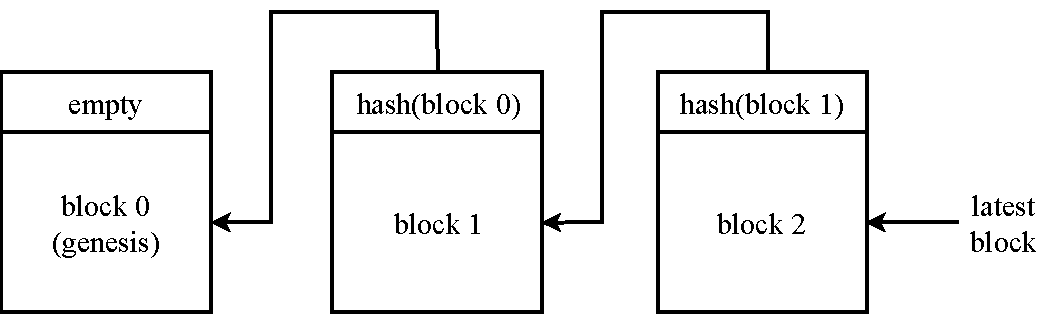
\includegraphics[scale=0.7]{figures/blockchain}
	\vspace*{0.25cm}
	\caption{Schematic representation of a blockchain. A blockchain is a list of blocks, connected to each other with an hash pointer. Each block contains a set of transactions.}
	\label{fig:blockchain}
\end{figure}


\subsection{Blocks}
Each block contains and confirms a number of transactions up to about \num{3000}.
By design, a new block is generated and appended to the blockchain every \num{10} minutes on average \cite{bitcoin_2008}.

The transactions inside each block are organized as a Merkle tree \cite{merkle_tree_1980}, a special binary tree with hash pointers (\cref{fig:merkle}).
The items in the tree are grouped in pairs and the hash of each of them is stored in the parent node.
The parent nodes are then grouped in other pairs and their hashed are stored in their parents:
this construction is repeated recursively until a single root node is created.
In the specific case of Bitcoin, each item in the tree represents a single transaction.

\begin{figure}[h]
	\centering
	\vspace*{0.1cm}
	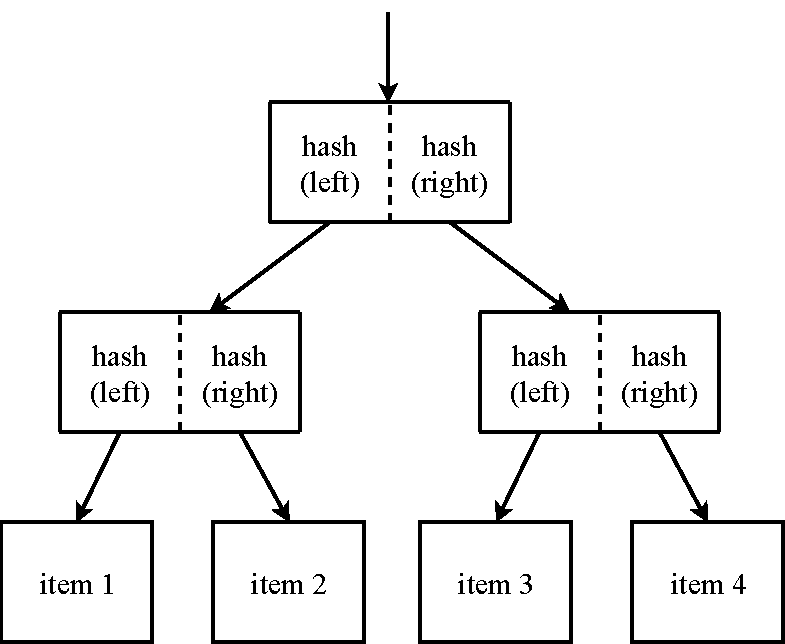
\includegraphics[scale=0.7]{figures/merkle}
	\vspace*{0.25cm}
	\caption{Schematic representation of a Merkle tree with \num{4} items.}
	\label{fig:merkle}
\end{figure}

The main advantage of using a Merkle tree is that the hash of the root uniquely identifies a specific set of transactions.
In fact, a change of a single item would modify the hashes of all ancestor nodes in the tree, thanks to the properties of the cryptographic hash functions.
This allows to divide a Bitcoin block in \num{2} parts - a header and a body - and distribute them independently of each other \cite{bitcoin_reference}.
The header contains only the hash of the Merkle tree root, the hash of the previous block in the blockchain and a couple of additional information such as protocol version and timestamp of creation.
The body stores the set the transactions as a serialized representation of the Merkle tree.

The second advantage of a Merkle tree is that transaction lookups in a block take $\mathcal{O}(n\log n)$ time, where $n$ is the number of transactions stored in the block.

Bitcoin blocks are distributed using a peer-to-peer protocol, which is explained in \cref{chapter:protocol}.


\subsection{Transactions}
TODO


\subsection{Addresses}
TODO: A Bitcoin address is similar to the concept a bank account:
it stores an amount of Bitcoin and is the only information required to make a payment to someone.
In contrast to traditional bank accounts, Bitcoin suggests to use each address only for a single transactions to preserve the privacy of the owner.
Each Bitcoin address corresponds to a pair of public and private key: the hash of the public key is the actual Bitcoin address, while the private key is needed to make payments using the bitcoins stored in the address.

\subsection{Wallets}
TODO

\subsection{Forks}
TODO

\subsection{Miners}
TODO

\subsection{Proof of Work}
TODO: PoW \cite{pow_2002}


\section{The Byzantine generals problem}
TODO: Bitcoin needs to ensure that everybody agrees on the quantity of money owed by each address.
To do so, each peer of Bitcoin stores the history of all transactions.
\cite{byzantin_generals_1982}
